\section{Application specification}
\label{sec:app:specification}
% 
% 
% \subsection{Bus load app}
% \label{app_specification:bus_load}
% Has the benefit of user adjustable provocation load rates for 
% further testing
% 
% The load app will provide different bus injection methods
% \subsubsection{Fault Injection via Buttons}
% Is the ability to inject faulty transmissions into the bus by pressing
% a button to check the fail-safetyness of the bus and the protocol.
% 
% This is meant to be the pendant of an electro magnetic disturbance
% injected into the bus cable and should be detected through the
% CRC sums by the receiver.
% 
% \subsubsection{Overload Simulation via Buttons}
% Is the ability to inject heavy bus load by pressing a button to
% check the accessibility of the bus if the bus is busy. 
% See also: \ref{app_specification:drift_rates} \nameref{app_specification:drift_rates}
% 
% \subsection{Drift rates}
% \label{app_specification:drift_rates}
% The main target of our application is to show drifts of the synchronous 
% clocks in our network. 
% 
% That means that we are measuring:
% \begin{itemize}
%  \item The ability of the nodes to synchronize the clocks via the bus 
% while it is under load due to the bus load application
%  \item The drifts between the clocks before synchronizing
% \end{itemize}
% 
% \subsection{Visualization of Drift Rates via LCD}
% The visualization is planned via a difference bar charts on the 
% LCD display of the uC board.
% 
% \subsection{Debugging and Monitoring features via PC}
% The ability to debug through the PC is one of the first 
% feature most developers are looking for. Therefore, it is an
% nice to have feature for us to engineer. 
% 
% This method could only unfold its full advantage in an emerging 
% developer version where the bus will be used in action.




The application is ment to run distributed 
as shown in figure \ref{fig:node_task_assignment} \nameref{fig:node_task_assignment}

\begin{figure}[ht]
 \centering
 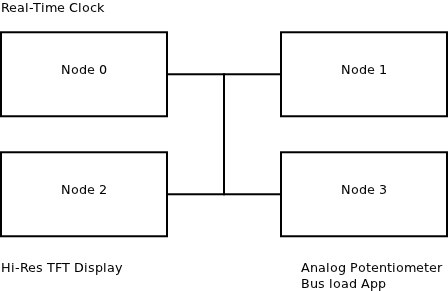
\includegraphics[scale=0.8]{../images/node_tasks.png}
 % node_tasks.png: 448x291 pixel, 72dpi, 15.80x10.27 cm, bb=
 \caption{Node task assignment}
 \label{fig:node_task_assignment}
\end{figure}


\subsection{Node2}
Node2 will take over the task of visualization described in
\ref{app_specification:drift_rates} \nameref{app_specification:drift_rates}

\subsection{Node3}
Node0 will take over the task of the bus load application
\ref{app_specification:bus_load} \nameref{app_specification:bus_load}